To support the key-value cache, each node must implement some form of indexing
service. Each indexing service must support a number of tasks such as
\emph{insertion}, \emph{deletion}, \emph{retrieval}, \emph{eviction} and
\emph{migration}. We consider three distinct but common indexing schemes:
\bptrees\cite{btree,bplustree}, Extendible Hashing\cite{ullman}, and
Counting Bloom Filters\cite{countingbloom1,countingbloom2}.

In order to operate in the elastic environment of our cache, when a node
overflows it must be capable of migrating a subset of its data records to
another node either preexisting or freshly allocated. Each of these schemes
have inherent differences in their structure and operation and, as such, are
compelling candidates for extension into the elastic makeup of \emph{Auspice}.

The remainder of this chapter will present background on each of the indexing
structures, describe the implementation of their migration mechanisms, and
provide an experimental analysis of their performance benchmarks.

\section{\bptrees} % (fold)
\label{sec:b_trees}
B-Trees and \bptrees are used in many of today's systems. The \bptree is a
multilevel indexing scheme that automatically adjusts the number of levels
depending upon the file size and stores all of its records in the leaf nodes.
Each record is stored in ascending order from left to right and each leaf node
is linked to the next and previous nodes. In this way, its design is
specifically crafted to accelerate queries over a range of
values\cite{navathe,ullman}. In terms of retrieval, \bptrees are balanced data
structures, where all paths from the root to any leaf have the same length
(similar to binary trees, with approximately log$_2 n$ depth).

\begin{figure}
\begin{center}
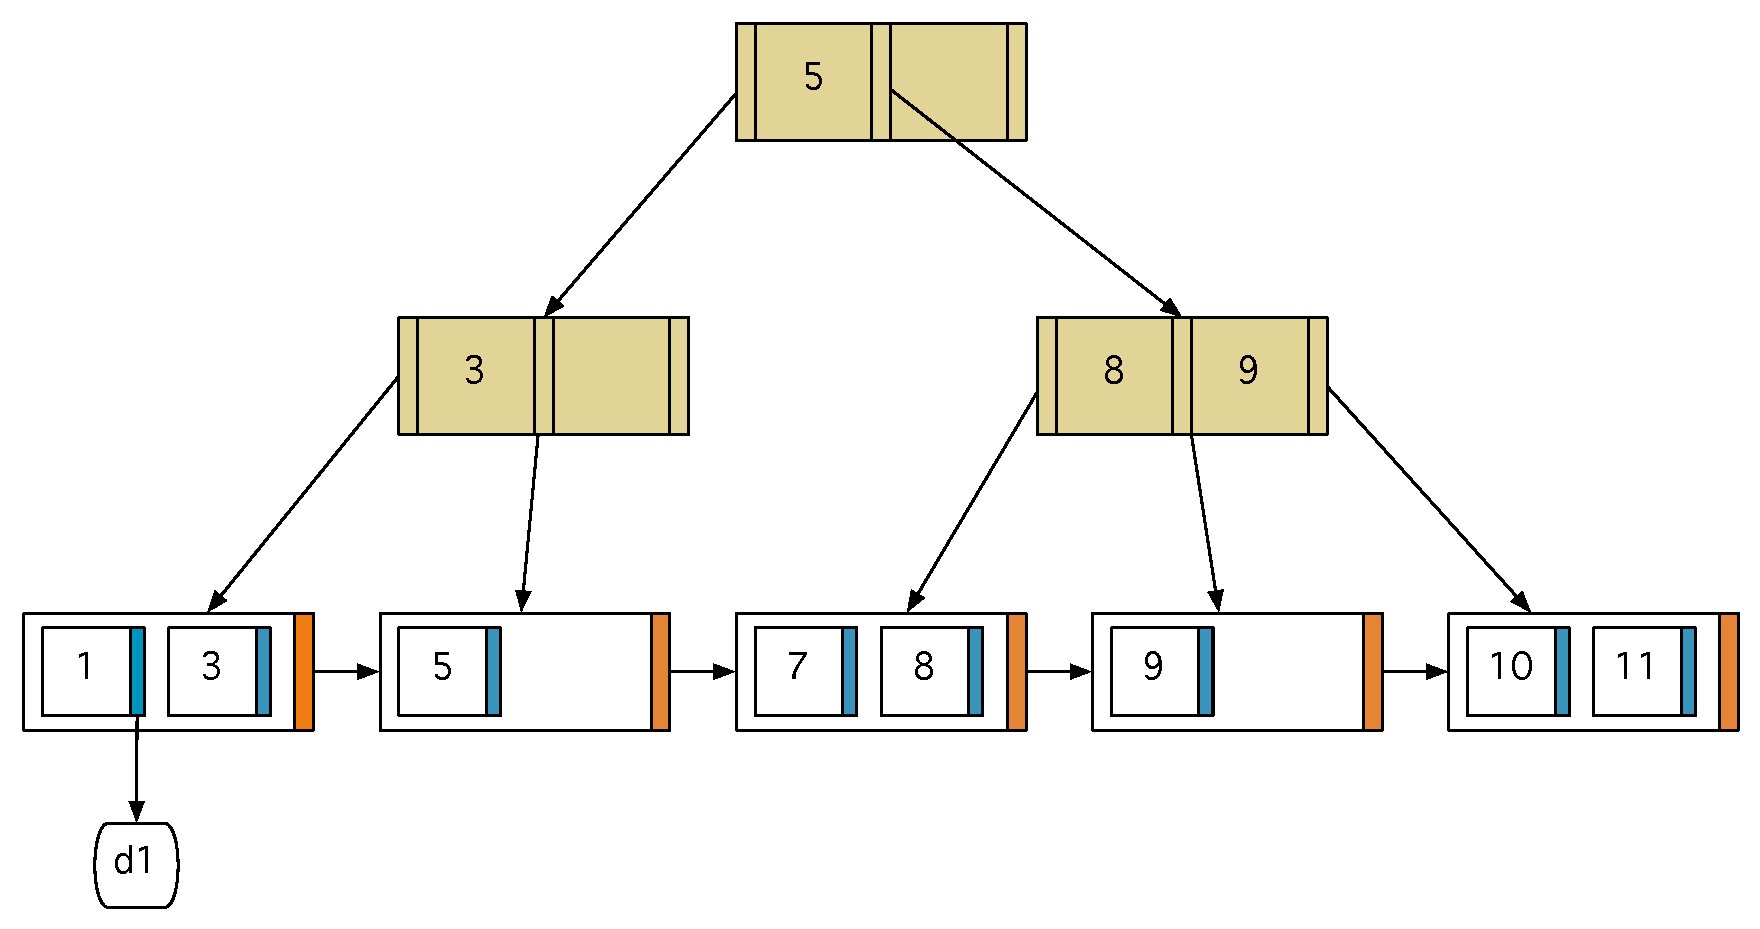
\includegraphics[scale=0.5]{figures/bplustree.pdf}
\end{center}
\caption{\bptree structure}
\label{fig:bplustree}
\end{figure}

Structurally, \bptrees are composed as shown in Figure~\ref{fig:bplustree}.
Internal nodes, those colored beige, act as pointers to other nodes in the
structure. All keys in the left branch of the key \emph{K} are less than or
equal to \emph{K}, while all keys to the right are greater than \emph{K}. While
searching, we compare the search key with the entries in the tree until such a
point as we reach the leaf node. Leaf nodes, those colored white, contain the
stored keys and pointers to the physical data location (blue). Additionally, in
order to assist with range queries, leaf nodes also contain a pointer to the
next leaf node, in order (orange).

With this sort of structure, we can see that range queries are made quite
simple and quick. Given a range $[k_{start}, k_{end}]$ we begin by searching to
find $k_{start}$ then proceed to iterate through the leaves until we find a
node greater than $k_{end}$. The search then returns the set of data identified
in that range. Due to this support, we expect the \bptree integration to be
well suited to elastic cache. Quick access to ranges of data should lead to
much faster data migration in the event of node additions. Data migration,
which is composed of a set of key deletions, can again be efficiently managed
in the same way as a range query is. The \bptree migration algorithm is shown
in Algorithm~\ref{alg:migrate1}.

\begin{algorithm}[htp]
\small
\caption{\label{alg:migrate1}BT\_Migrate($k_{start}$, $k_{end}$)} \begin{algorithmic}[1]
\STATE $\triangleright$ manipulate B$^+$-tree index and transfer the keys in form of a string, $keys$
\STATE $end \leftarrow false$
\STATE $\triangleright$ $L =$ leaf initially containing $k_{start}$ 
\STATE $L \leftarrow btree$.search($k_{start}$)
\WHILE{$(\neg end \wedge L \neq NULL)$}
 \STATE $\triangleright$ each leaf node contains multiple keys
 \FORALL {$(k,v) \in L$}
   \IF {$k \le k_{end}$}
     \STATE $keys$.append($k$, $v$)
     \STATE $btree$.delete($k$)
   \ELSE
     \STATE $end \leftarrow true$
     \STATE break
   \ENDIF
 \ENDFOR
 \STATE $L \leftarrow L$.next()
\ENDWHILE
\STATE return $keys$
\end{algorithmic}
\end{algorithm}

% TODO: This section is cribbed heavily from IJNGC paper, look at rewrite.

% section B_Trees (end)

\section{Extendible Hashing} % (fold)
\label{sec:extendible_hashing}
Hash tables are another ubiquitous form of indexing and are often a favorite
tool of developers looking for key-value storage. These structures excel at
offering constant-time searches, unlike the logarithmic searches of \bptrees.
However, there is a tradeoff in that hash tables are not well-equipped to
handle range queries.

In most hash implementations, we assume there is some hash function $h(k)
\exists [0, B-1]$, where $B$ is the total number of buckets stored in the
table. Each bucket then contains a set of records, stored either in memory or
in secondary storage. Ideally, a hash function maps each key to a distinct
bucket. In practice however, this is seldom possible as the key range is
significantly larger than $B$. Therefore, the buckets typically allow for the
storage of a set of records. Even still, they can overflow. To avoid this, hash
tables implement some form of collision resolution. One of the most simple
techniques is to have the bucket overflow into a chain. Records mapping to an
already occupied bucket are stored in a linked list format attached to that
bucket. This performance of this solution degrades linearly as the number of
records $K$, and more importantly, the ratio of $K$ to $B$ increases.

We can avoid this problem by using dynamic hashing\cite{dh2}, where the number
of buckets, $B$, is variable. In dynamic hashing schemes, $B$ is increased whenever
necessary. For the purposes of our elastic cache, we have implemented a form of
dynamic hashing called Extendible Hashing\cite{dh1}, which introduces the
concept of a \emph{directory} -- an array of pointers to the hash buckets. The
buckets then contain an additional array of pointers to the physical location
of the records.

Initially, each directory contains a single bucket and is allowed to grow
when required. In Extendible Hashing, the length of the directory is always a
power of two, which means that each growing phase doubles the size of the
directory. Because multiple pointers can reference the same physical bucket,
the number of actual buckets can be less than or equal to the size of the
directory. A hash function $h(k)$ computes a binary sequence for each record
based on the search key, $k$, and the first $i$ least significant bits are used
to determine the bucket to which the record belongs. When a directory contains
$2^i$ pointers to buckets, the actual number of buckets is $\leq 2^i$.

Searching for a key in an extendible hash table is done in two steps. First,
the hash function is run over the key, and the least significant $i$ bits are
used to determine the bucket the key belongs to. Once the bucket has been
identified, a linear scan is run over the contents of the bucket to return the
position of the record, if found. Again, the search time increases as the
number of records per bucket increases. A large number of records per bucket is
also indicative of fewer splits and a smaller directory. As the directory size
increases, the number of records per bucket should thin out in the general
case. As mentioned earlier, while Extendible Hashing offers $O(1)$ time
exact-match queries, range queries suffer as the hash function disrupts $k$'s
original locality.

To support migration, we implemented Extendible Hashing in such a way that we
could dynamically specify the number of records per bucket. Because Extendible
Hash tables do not store the records in a particular order, we must linearly
scan through each bucket and delete keys that lie within the migration range.

The migration procedure takes as input, the range of keys to be migrated,
$[k_{start}, k_{end}]$. We begin by traversing all directories, and for each
directory we follow the pointer to its corresponding bucket. Any key, $k$, which
lies in the migration range is appended, along with its data object, to an
array. This array is returned once all records have been scanned. This
process is shown in Algorithm~\ref{alg:migrate2}.

\begin{algorithm}[htp]
\small
\caption{\label{alg:migrate2}EH\_Migrate($k_{start}$, $k_{end}$)} \begin{algorithmic}[1]
\STATE static $H$ $\triangleright$ bring extendible hashtable to scope
\STATE $keys \leftarrow \{\}$
\FOR {$x \leftarrow 0$ to  $2^i-1$}
  \STATE $D_x \leftarrow H$.getDirectoryAt($x$)
 \FOR {$y \leftarrow 0$ to $|D_x|-1$}
   \STATE $B_y \leftarrow D_x$.getBucketAt($y$)
   \FORALL {$k \in B_y | k \ge k_{start} \wedge k \le k_{end}$}
       \STATE $keys \leftarrow keys \cup~(k,v)$
       \STATE $H$.delete($k$)
   \ENDFOR
 \ENDFOR
\ENDFOR
\STATE return $keys$
\end{algorithmic}
\end{algorithm}

% section extendible_hashing (end)

\section{Bloom Filters} % (fold)
\label{sec:bloom_filters}

Bloom Filters\cite{bloomfilter1} are probabilistic data structures used to
quickly determine the membership of a record in a set. It is composed of a
$m$-bit length bit array and a set of $j$ hash functions, each of which hashes
a set element to one of the $m$ different values. Generally, $m \gg j$, which
reduces the probability of the hash function setting the same bit for a record.
Though Bloom Filters are vulnerable to false positives, false negatives are not
possible.

Insertions into a Bloom Filter are simple: apply the hash function to the key
and set the corresponding bits. Determining membership is also simple: apply
each of the $j$ hash functions to the key and verify if the corresponding bits
are set. If any of the $j$ bits are not set, then the element is not present.
However, because false positives are possible, even if each of the bits are
set, the record may still not be present, and so a scan becomes necessary after
a pseudo-hit. Fortunately, the false positive rate has a bound $f = (1 -
e^{(-jN/m)})^j$, where $j$ is the number of hash functions, $m$ is the length
of the bit array, and $N$ is the number of set bits. From this, we can clearly
see that the false positive rate increases as the number of inserts increases.
By choosing a relatively large $m$ and independent hash functions, we can
render the false positive rate negligible\cite{falsepositive}.

Traditionally, Bloom Filters disallow deletions as the same bit can be set for
multiple records. By modifying the bit array, false negatives would become a
possibility, which are prohibitive. To support deletion, we implemented a
variant called Counting Bloom Filters\cite{countingbloom1,countingbloom2}. Each
bit in the bit array is associated with a 4-bit counter, which then keeps track
of the number of records that set the bit. This counter enables the delete
operation.

These structures are most useful for applications that require fast tests of
record existence, and especially beneficial for those that test non-existence.
To search for a record with key $k$, we apply the $j$ hash functions to $k$. We
then $AND$ all bits from the bit array corresponding to the locations $h_i(k) |
i = (0,\ldots,j)$. If the result of this operation is one, then the record may be
present and a scan is performed to retrieve the record. If the result is zero,
the record is non-existence. Because a linear scan may be required for a hit,
there is a costly overhead involved in the case of false positives. However, as
mentioned, low false positive rates can be ensured by having a large $m$ and
independent hash functions.

Implementing migration in a Counting Bloom Filter is also quite simple. Again
we operate over the range $[k_{start},k_{end}]$. We begin from the minimum
threshold and increment until we reach the maximum threshold, searching for
each key in the range. Keys that are present are then deleted. This makes
migration time linear to the amount of keys within $[k_{start},k_{end}]$. This
algorithm is demonstrated in Algorithm~\ref{alg:migrate3}.

\begin{algorithm}[htp]
\small
\caption{\label{alg:migrate3}CBF\_Migrate($k_{start}$, $k_{end}$)} \begin{algorithmic}[1]
\STATE static $H$ $\triangleright$ counting bloom filter to scope
\STATE $keys \leftarrow \{\}$
\FOR {$k \leftarrow k_{start}$ to  $k_{end}$}
  \IF {$H$.contains($k$)}
    \STATE $v \leftarrow H$.retrieve($k$)
    \IF {$v \neq$ NULL}
      \STATE $keys \leftarrow keys \cup~(k,v)$
    \ENDIF
  \ENDIF
\ENDFOR
\STATE return $keys$
\end{algorithmic}
\end{algorithm}
% section bloom_filters (end)

\section{Elastic Cache Support} % (fold)
\label{sec:elastic_cache_support}
We have implemented this system on EC2 and here we describe the system within
that context. The Amazon Elastic Compute Cloud (EC2) supports
Infrastructure-as-a-Service (IaaS), allowing users to allocate nodes on demand.
EC2 nodes (\emph{instances}) are virtual machines that can launch system
snapshots (\emph{images}). These virtual machines are deployed onto various
architectures (\emph{instance types}) with varying costs depending upon their
capabilities. As a baseline, we have chosen to use only small instances in our
implementation, though there are instances with far greater (and fewer)
capabilities available.

During system execution, records may continually be inserted into the cache
nodes. Overflow of any individual node may invoke an incremental scaling
effort. This process involves starting a new EC2 node and migrating a subset of
the data from the overflown node to the newly allocated node. There are two
areas of overhead in this process: (1) instance allocation time, which can take
up to several minutes during peak time, and (2) data migration time, which
involves identifying the migration range and network transfer time.

In our experience, instance allocation time dominates that of data migration.
We thus, implement a system that pre-launches instances speculatively when some
threshold, $T$, has been met. At background thread initiates the pre-launching
and begins to eagerly migrate data from the fullest node once the new one has
been booted. Out threshold $T$ is based on the following observations: if the
request rate is high, then $T$ should be lowered, as the nodes are likely to
fill up faster. Conversely, if the request rate is low, then $T$ should be
raised. If $n$ is the node to insert some $(k,v)$ pair, we use the following to
estimate $n$'s threshold.
\begin{center}
  $T = c(n)/2 + \delta_H \times (||N|| - R/\delta_L)$
\end{center}
where $\delta_L$ and $\delta_H$ are constants: the lowest and highest
\emph{expected} querying rate respectively. $R$ is the current request rate,
$c(n)$ is the capacity of node $n$ and $||N||$ is the total number of nodes in
our cache. As the number of nodes, $||N||$ increases, the threshould should
also increase so as to delay the allocation of new nodes. $R/\delta_L$ is used
to normalize the current rate, $R$.

We use this threshold in our cache insertion algorithm, shown in
Algorithm~\ref{alg:optimize}. The identifiers used in
Algorithm~\ref{alg:optimize} are listed in Table~\ref{tab:vars1}.

\begin{table}[htp]
\caption{\label{tab:vars1}Listing of Identifiers for Algorithm~\ref{alg:optimize}}
\centering
\begin{tabular}[]{| c || p{5.5cm} |}
  \hline
  \textbf{Identifier} & \textbf{Description} \\
  \hline
  \hline

  $k$ & A queried key \\
  \hline
  $B = (b_1, \ldots, b_p)$ & The list of all buckets on the hash line\\
  \hline
  $h(k)$ & The hash function, which returns the closest upper bucket to $k$ \\
  \hline
  $N =(n_1, \ldots, n_m)$  & The set of all nodes in the cooperative cache \\
  \hline
  $n \in N$  & A cache node  \\
  \hline
  $||n||$  & Current size of index on node $n$  \\
  \hline
  $\lceil{n}\rceil$  & Overall capacity on node $n$ \\
  \hline
 $||N||$  & Number of nodes part of the cooperative cache $N$  \\
  \hline
  $R$  & Query intensity, i.e.\ queries per time step  \\
\hline
  \end{tabular}
\end{table}

\begin{algorithm}[htp]
\small
\caption{\label{alg:optimize}Speculative-Insert($k$, $v$, $\delta_L$,
$\delta_H$)} \begin{algorithmic}[1] \STATE static $NodeMap[\ldots]$
\STATE static $B = (\ldots)$
\STATE static $h' : K \rightarrow [0,r)$
\STATE $n \leftarrow NodeMap[h'(k)]$
\STATE $T = c(n)/2 + \delta_H \times (||N|| - R/\delta_L)$
\IF {$T < \lceil{n}\rceil \times 0.1$}
	\STATE $T \leftarrow \lceil{n}\rceil \times 0.1 $\ \ \ \ $\triangleright$ to avoid
	extremely low values of threshold
\ENDIF
\IF {$T > (\lceil{n}\rceil \times 0.75) $}
	\STATE $T \leftarrow \lceil{n}\rceil \times 0.95$\ \ \ \ $\triangleright$ to delay
	allocation of new nodes
\ENDIF

\IF {$||n|| + sizeof(v) < T$}
	\STATE $n$.insert($k,v$)\ \ \ \ $\triangleright$ insert directly on node $n$
\ELSIF{$||n|| + sizeof(v) > T$}
	\STATE $\triangleright$ Launch threads $t1,t2$ which would execute the Lines 16 - 22
	\STATE $\triangleright$ find fullest bucket referencing $n$
	\STATE $b_{max} \leftarrow
		\underset{b_i \in B}{\operatorname{argmax}} ||b_i|| \wedge NodeMap[b_i] = n$
	\STATE $k^{\mu} \leftarrow \mu(b_{max})$
	\STATE $n_{dest} \leftarrow n$.migrate($min(b_{max})$, $k^{\mu}$)
	\STATE $\triangleright$ update structures
	\STATE $B \leftarrow (b_1, \ldots, b_i, h'(k^{\mu}), b_{i+1}, \ldots,
	b_p)~|~b_i < h'(k^{\mu}) < b_{i+1}$
	\STATE $NodeMap[h'(k^{\mu}))] \leftarrow n_{dest}$
\ELSE
	\STATE $\triangleright$ $n$ overflows
	\STATE $\triangleright$ Launch Thread $t3$ if $t1$ and $t2$ are not taking care of $n$ and execute Lines 16-22
\ENDIF

\end{algorithmic}
\end{algorithm}

% TODO: Algorithm explanation (see IJNGC)

% section elastic_cache_support (end)

\section{Experiments} % (fold)
\label{sec:experiments_indexing}

% section experiments_indexing (end)

\section{Results} % (fold)
\label{sec:results_indexing}

% section results_indexing (end)
